\subsection{29. Конечные преобразователи и задаваемые ими преобразования. Различные варианты определения. Примеры конечных преобразований. Теорема Нива.}

\Def Конечный преобразователь $T = \langle Q, \Sigma, \Gamma, \Delta, q_0, F \rangle$:

\begin{enumerate}
    \item $Q$ — множество состояний, $|Q| < \infty$;
    \item $\Sigma$ — входной алфавит, $|\Sigma| < \infty$;
    \item $\Gamma$ — выходной алфавит, $|\Gamma| < \infty$;
    \item $\Delta \subset (Q \times \Sigma^*) \times ( Q \times \Gamma^*)$ — множество переходов;
    \item $q_0 \in Q$ — стартовое состояние;
    \item $F \subset Q$ — множество завершающих состояний. Можно считать, что $|F| = 1$
\end{enumerate}

\Def Конфигурация КПтеля $T$ -- это тройка $\angles{q, u, v}\ \ (q \in Q, u \in \Sigma^*, v \in \Gamma^*) $
\newline \textit{Неформально:} находимся в состоянии $q$; осталось прочесть слово $u$; вывели слово $v$

\Def Отношение выводимости $(\vdash)$ -- наименьшее рефлексивное транзитивное отношение, что:
$$
\forall \angles{q_1, u} \rightarrow \angles{q_2, v} \in \Delta \text{ выполнено: } \forall y \in \Sigma^*,\; z\in\Gamma^* : \angles{q_1,uy,z} \vdash \angles{q_2,y,zv}
$$

\Def Соответсвие, задаваемое конечным преобразователем $T$:
$$
\psi = \{(u,v) \in  \; | \; \exists q\in F \, : \, \angles{q_0, u, \varepsilon} \vdash \angles{q, \varepsilon, v}\}
$$

\Def Конечное преобразование (КП) -- это $\psi : \Sigma^* \rightarrow \Gamma^*$

\begin{figure}[h!]
    \centering
    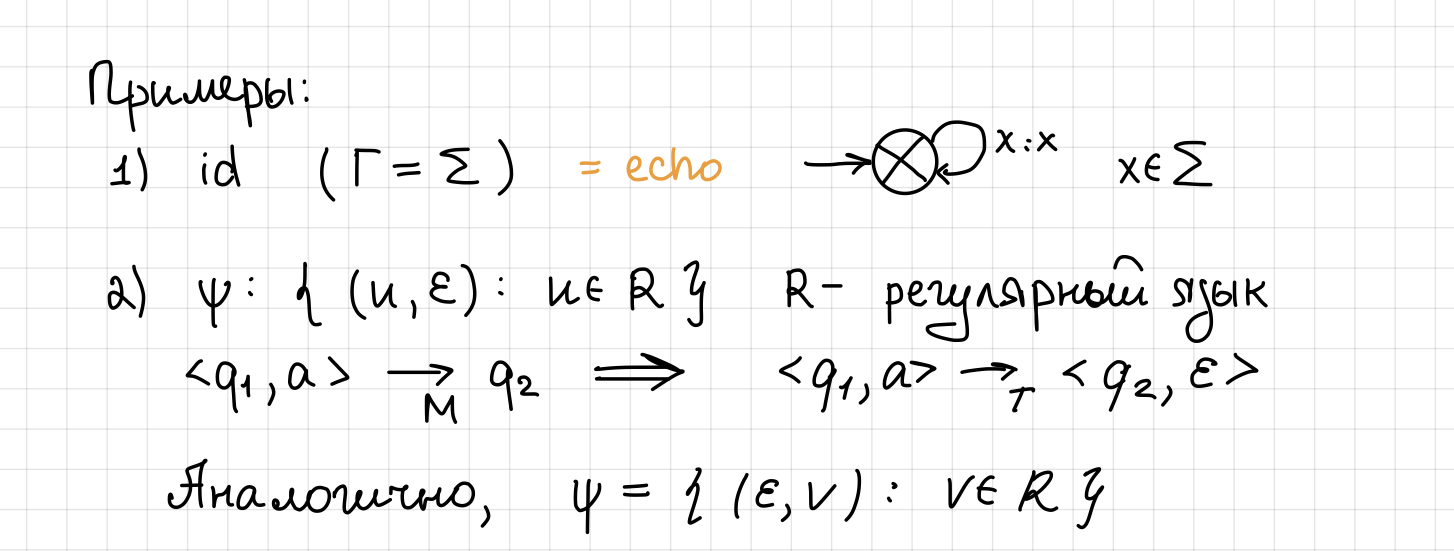
\includegraphics[scale=0.35]{KP_ex1.PNG}
\end{figure}
\newpage
\begin{figure}[h!]
    \centering
    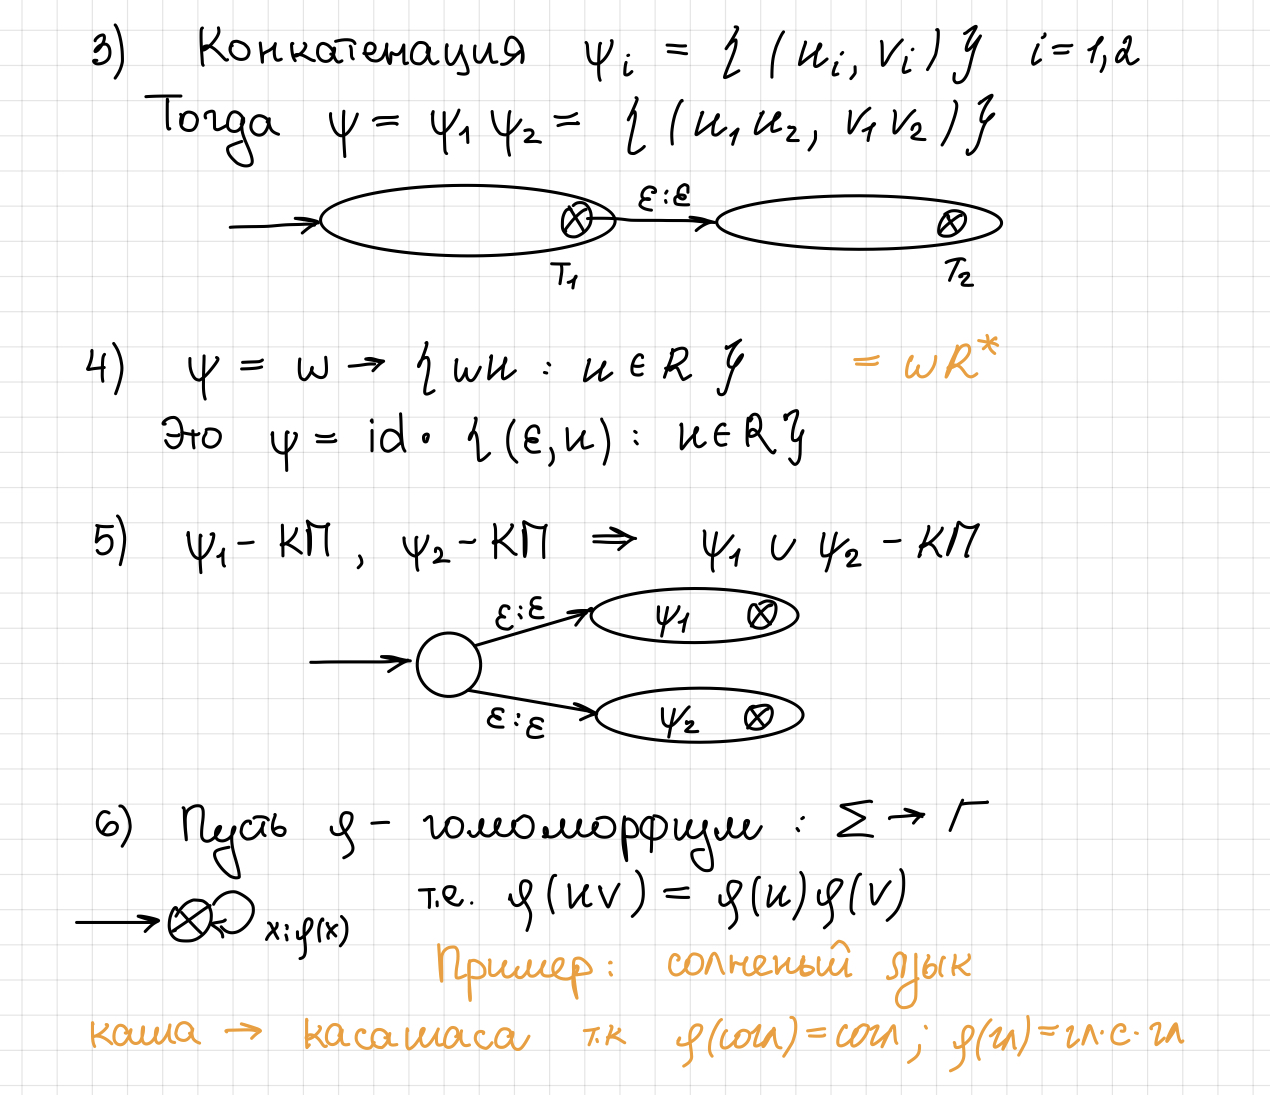
\includegraphics[scale=0.35]{KP_ex2.PNG}
\end{figure}

\Def Неудлиняющий гомоморфизм -- это $\psi :\, \forall x\in\Sigma^* \;\; |\psi(x)| \leqslant |x| $

\Lemma $\forall T = <Q, \Sigma, \Gamma, \Delta, q_0, F> \exists$ эквивалентный ему $T' = <Q', \Sigma, \Gamma, \Delta ', q_0, F'>:$

$\forall <q_1, u> \to <q_2, v> \in \Delta ': |u| + |v| = 1$.

\Proof
Аналогично НКА.

$u = u_1 u_2 \dots u_k, v = v_1 v_2 \dots v_m$.
Добавим состояния и переходы вида $u_i:\varepsilon$ и $\varepsilon:v_j$.

\begin{minipage}[r]{0.15\linewidth} 
%\begin{flushright}
    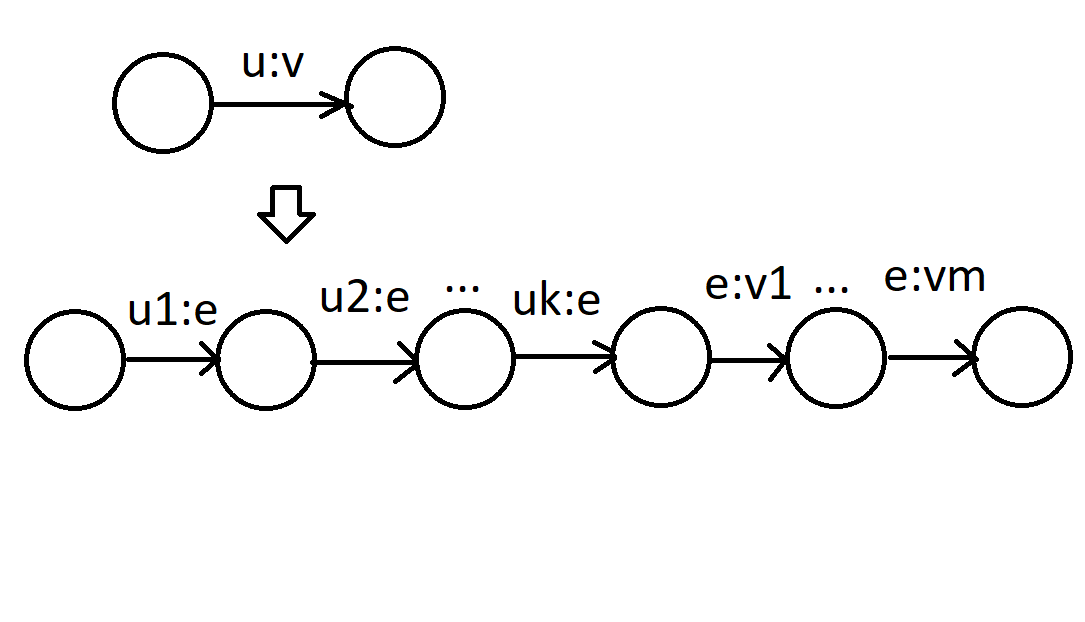
\includegraphics[width=2\linewidth]{images/29_5.png}
%\end{flushright} 
\end{minipage} \\

Осталось убрать переходы вида $\varepsilon:\varepsilon$ (не забываем корректно проставить завершающие состояния) :

\begin{minipage}[r]{0.15\linewidth} 
%\begin{flushright}
    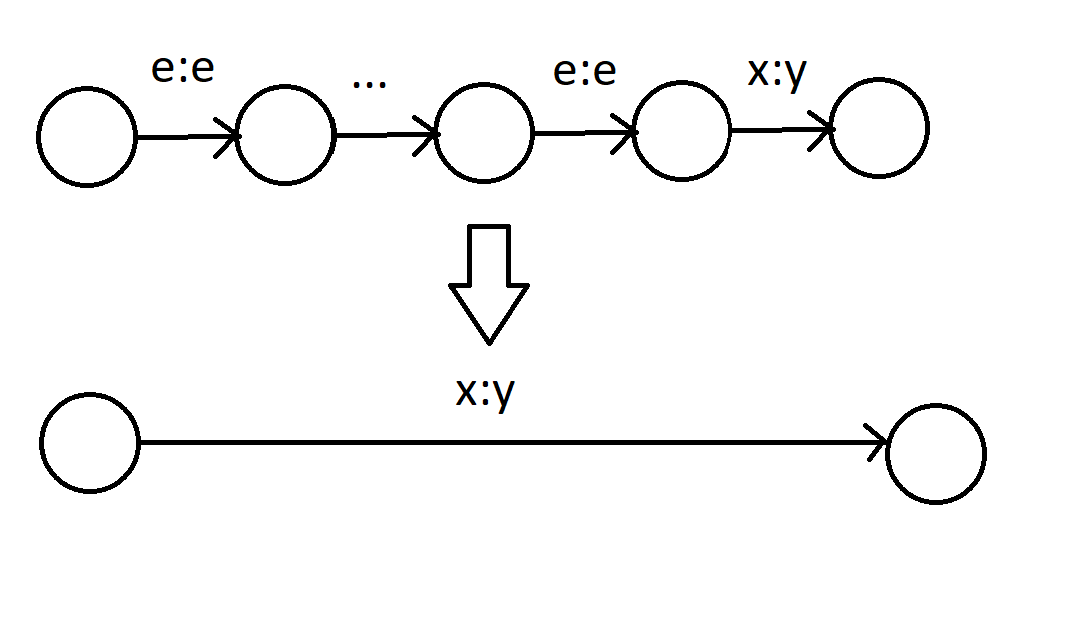
\includegraphics[width=2\linewidth]{images/29_6.png}
%\end{flushright} 
\end{minipage} \\

\EndProof

\textbf{Теорема Нива:} Любое конечное преобразование можно представить в виде композиции: 
\begin{itemize}
    \item обратного неудлиняющего гомоморфизма: $\psi^{-1} : \Theta^* \rightarrow \Sigma^*$
    \item ограничения на регулярный язык: $id_R \;\; R \subset \Theta^*$
    \item неудлиняющего гомоморфизма: $\eta : \Theta^* \rightarrow \Gamma^*$
\end{itemize}

\Proof
Если $\psi$ -- КП, то существует конечный преобразователь $M : L(M) = \psi$ т.ч. $|u| + |v| = 1$.

Пронумеруем ребра конечного преобразователя $M: e_1, e_2, \dots, e_n$

$\Theta = \{e_1, e_2, \dots, e_n\}$

$R$ -- все пути из $q_0$ в $F$. Заметим, что язык автоматный т.к. на каждом ребре написан символ, ему соответствующий. Поэтому он и регулярный.

$\phi$ -- для каждого ребра берем вход, $\eta$ -- для каждого ребра берем выход

Заметим, что $\phi$ и $\eta$ неудлиняющие т.к. $|\phi(x)| \leq 1 \forall x \in \Theta$ т.к. на переходах не более одной буквы.

Докажем теперь про композицию.

$\psi = (u, v)$

Рассмотрим автомат над $\Theta$, который мы получаем, когда расписываем все по однобуквенным переходам и нумеруем ребра. В нем есть какой-то путь из $q_0$ в $q \in F$, пройдя по которому, мы $u$ преобразуем в $v$, то есть:

$\angles{q_0, e_{i1} \dots e_{ik}} \vdash \angles{q, \varepsilon}$. Заметим, что тогда $e_{i1}, \dots, e_{ik} \in R$, поэтому $id$ его не изменит (оставит).

$\phi(e_{i1} \dots e_{ik}) = u,\;\; \eta(e_{i1} \dots e_{ik}) = v$ (из определения $\phi$ и $\eta$).

Поэтому для $\psi = (u, v) \Rightarrow \exists q \in F: \angles{q_0, u, \varepsilon} \vdash_k \angles{q, \varepsilon, v}$.
\EndProof

\textbf{Пример:}

\begin{minipage}[r]{0.15\linewidth} 
%\begin{flushright}
    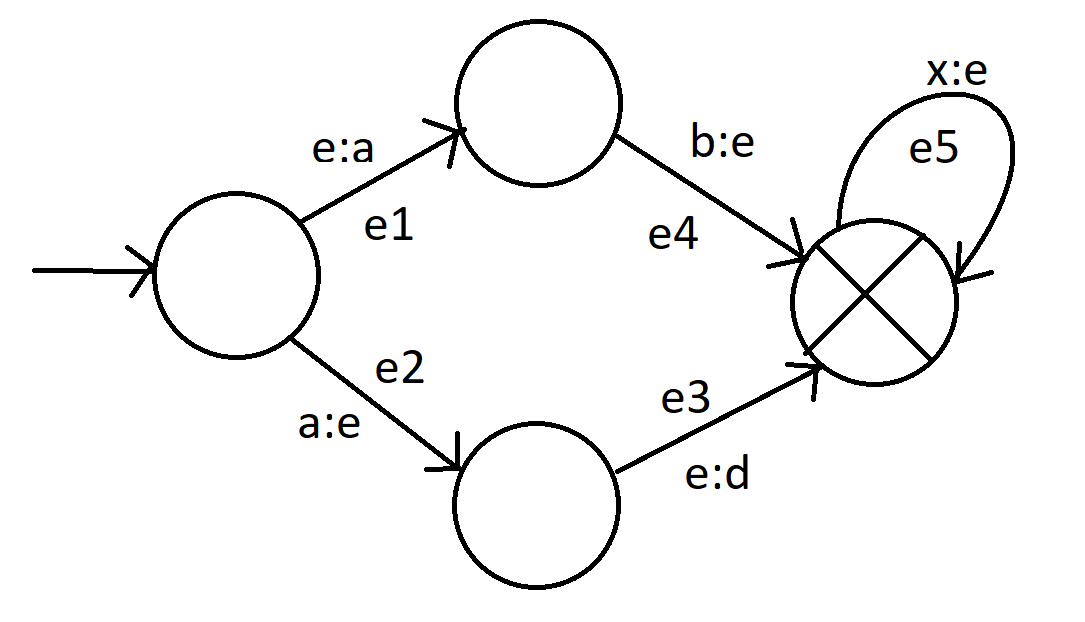
\includegraphics[width=2\linewidth]{images/29_7.png}
%\end{flushright} 
\end{minipage} \\

$\Theta = {e_1, e_2, e_3, e_4, e_5}$, 

$R = (e_1 e_4 + e_2 e_3)e_5^*$

$\phi(e_1) = \varepsilon, \phi(e_2) = a, \phi(e_3) = \varepsilon, \phi(e_4) = b, \phi(e_5) = x$

$\eta(e_1) = a, \eta(e_2) = \varepsilon, \eta(e_3) = d, \eta(e_4) = \varepsilon, \eta(e_5) = \varepsilon$